% Converted from README.md
\paragraph{Primer: Studenti}\label{primer-studenti}

Program učitava imena i prezimena studenata iz datoteke \texttt{students.txt} i predmete iz datoteke \texttt{subjects.txt} i potom ispisuje informacije o studentima i prosečnim ocenama, po predmetu i u globalu. Ukupno 100 studenata sa po 100 ocena iz svakog od 40 predmeta. Spiskovi sa studentskim rezultatima ispisuju se 10 puta. Analiziramo program Callgrind-om:

\begin{minted}{bash}
$ valgrind --tool=callgrind --cache-sim=yes ./students.out
\end{minted}

Otvaramo izveštaj u KCachegrind-u. Gledamo sa leve strane broj pozivanja svake funkcije i broj instrukcija koji je zahtevalo njeno izvršavanje, samostalno i uključujući izvršavanja drugih funkcija koje je pozivala. Sa desne strane možemo izabrati prikaz mape poziva i sa izborom \emph{All Callers}, videćemo koje su sve funkcije pozivale funkciju od interesa.

\pandocbounded{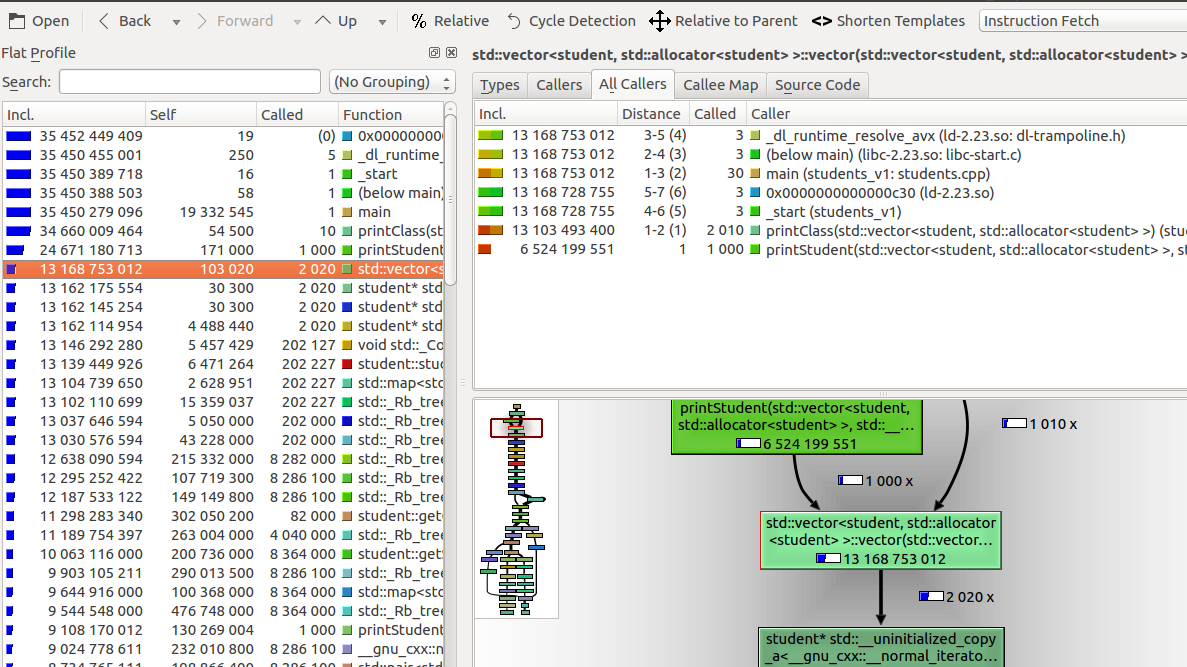
\includegraphics[keepaspectratio]{images/call1_1.png}}

Zanima nas zašto se funkcija iz standardne biblioteke poziva 2020 puta. Ako iz alata pogledamo izvorni kod, videćemo da se pri samom početku funkcije \texttt{printClass} konstruktor kopije za \texttt{std::vector} poziva 10 puta. To je broj generisanja izveštaja i broj poziva ove funkcije. Problem je što se ceo vektor studenata u funkciju prenosi po vrednosti, a ne po referenci. Zato se prilikom svakog poziva kreira kopija za konkretan poziv. Izmenimo kod i primetno ćemo ubrzati izvršavanje programa.
